\section{Learning Pong}
\label{sec:pong}
The most widely used approach to implementing a learning agent that plays Pong is deep reinforcement learning.
Since the introduction of DQNs, standard methods have been used less and less as they cannot easily handle large inputs.

% TODO: aggiungere parte su algoritmi genetici

Mnih, Volodymyr, et al. \cite{mnih2013playing} introduced the concept of Deep Q-Network, a convolutional neural network, trained with a variant of Q-learning.
Seven popular ATARI games were considered in this work, including Pong.
%
Grayscale game frames are captured at 210x160 resolution, downsampled to a 110x84 image and cropped to an 84x84 patch.
%
The network has an input shape of $84\times 84\times k$, where $k$ is the number of skipped frame and has a separate output unit for each possible action, 
the number of which depends on the game considered. 
For all games considered all positive rewards are fixed at 1 and all negative rewards at -1.
%
The network is trained with an $\epsilon$-greedy annealed strategy and a replay memory of most recent frames is used to ease the training.

Another work that uses DQN focusing on Pong is \cite{makarov2017learning}, which use an episodic control technique \cite{blundell2016model} to reuse successful
strategies.
%
The screenshots are taken at 32 FPS binarized and rescaled to 80x80, and the reward considered is the same as in \cite{mnih2013playing}.
The agent actions considered are: move paddle up, move paddle down and paddle stays at the same place.

Diallo et al. \cite{diallo2017learning} discusses the emergence of cooperative and coordinated behaviors between joint and concurrent learning
agents using deep Q-learning. 
%
In the considered scenario, two agents form a team to win against an hard-coded AI,
and learn how to cooperate and how to divide the field.
%
As in \cite{mnih2013playing}, the images are resized to 84x84 and a frame skip of 4 is used.
Experience replay is also used.
%
There are three actions that each agent can take: move up, move down, stay at the same place (\cref{tab:reward-scheme}).

\begin{figure}[ht]
  \centering
  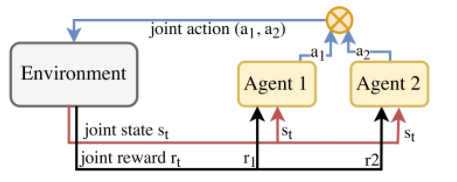
\includegraphics[width=0.4\textwidth]{images/DQN_MAS.png}
  \caption{Multi-agent concurrent DQN \cite{diallo2017learning}.}
  \label{fig:dqnmas}
\end{figure}

\begin{table}[ht]
  \renewcommand{\arraystretch}{1.3}
  \caption{Reward scheme adopted by \cite{diallo2017learning}.}
  \label{tab:reward-scheme}
  \centering
  \begin{tabular}{@{}ccc@{}}
    \toprule
    \textbf{Events}            & \textbf{Agent 1 reward} & \textbf{Agent 2 reward} \\ \midrule
    \textbf{Left player loses} & +1                      & +1                      \\
    \textbf{One agent loses}   & -1                      & -1                      \\
    \textbf{Collision}         & -1                      & -1                      \\ \bottomrule
  \end{tabular}
\end{table}

Unlike previous works where the agent learns to play Pong against a hard-coded AI, 
Tampuu, Ardi, et al. \cite{tampuu2017multiagent} have considered both as learning agents and have shown that different rewarding schemes lead them towards competition or collaboration.
%
Multiple agents controlled by autonomous DQNs learn to cooperate and compete while sharing a high-dimensional environment and being fed only raw visual input \cite{tampuu2017multiagent}.
%
Each of the two agents can take four actions: 
move up, move down, stand still, and fire (to relaunch the ball or to start the game).
%
Three rewarding schemes were studied (\cref{tab:reward-scheme-2}).
%
\begin{table}[ht]
  \renewcommand{\arraystretch}{1.3}
  \caption{Rewarding schemes to explore the transition from competitive to the cooperative strategy \cite{tampuu2017multiagent}. Fully competitive $\rho = 1$, fully cooperative $\rho = -1$, intermediate $\rho = range(-1, 1, 0.25)$.}
  \label{tab:reward-scheme-2}
  \centering
  \begin{tabular}{@{}ccc@{}}
    \toprule
                                                   & \textbf{Left player scores} & \textbf{Right player scores} \\ \midrule
    \multicolumn{1}{c}{\textbf{Left player scores}} & $\rho$                   & -1                       \\ 
    \multicolumn{1}{c}{\textbf{Right player scores}} & -1                       & $\rho$                   \\ \bottomrule
  \end{tabular}
\end{table}

McBrien et al. \cite{mcbrien2020learning} proposed a different approach which uses a neural network automatically generated with genetic algorithms to allow agents to learn how to play Pong.
%
A custom version of Pong is considered where the goals are smaller and the players have the ability to move in both the x and y dimensions.
%
The state is represented as eight inputs: the paddle's X and Y position, the opponent's X and Y position, the ball's X and Y velocity,
and the ball's X and Y position and the output of the neural network has four output nodes for each possible action: up, down, left and right.
%
Two algorithms were used: NeuroEvolution(NE) and NeuroEvolution of Augmenting Topologies(NEAT).
The first start from a predefined neural net structure and iteratively tune its parameters, while the second adds the possibility to modify the network topology by adding nodes and connections randomly.

\begin{figure}[ht]
  \centering
  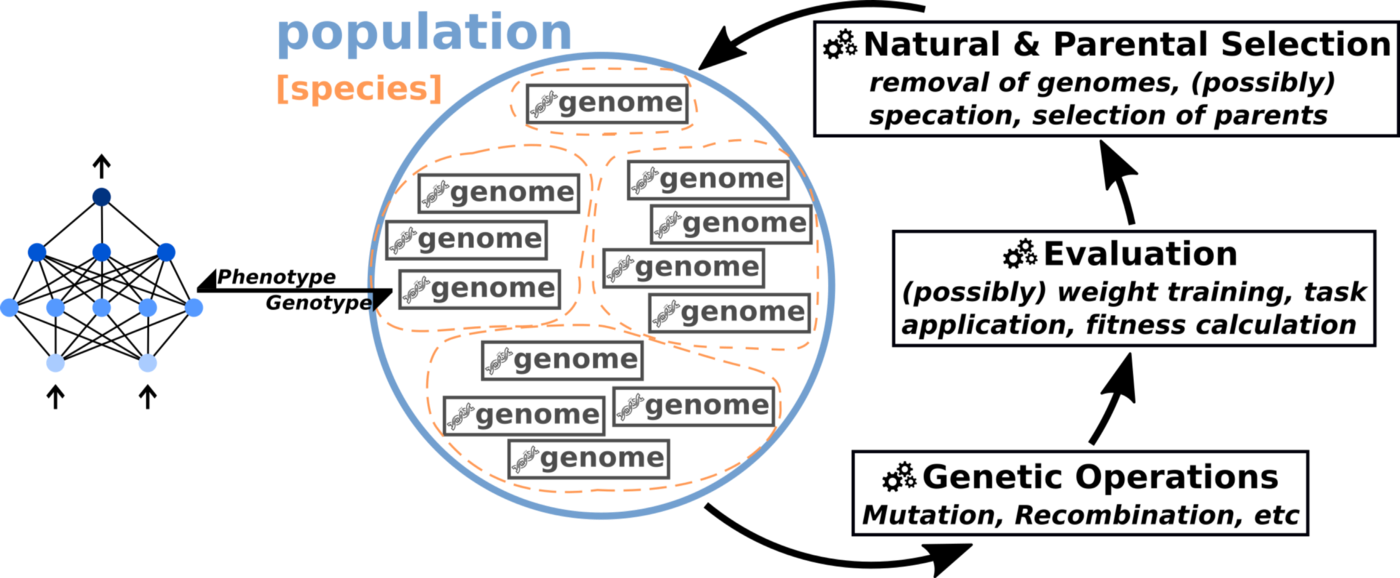
\includegraphics[width=0.4\textwidth]{images/neuroevolution.png}
  \caption{NeuroEvolution algorithm schema.}
  \label{fig:ne}
\end{figure}
